%\chapter{Vorlesung}
%\section{Vergleichsbasierte Sortieralgorithmen}
\pagebreak
\section{Worst-case Laufzeit}
Worst-case Laufzeit eines vergleichsbasierten Sortieralgorithmus \\$~\hat{=}~$ maximale Tiefe des zugehörigen Entscheidungsbaums \\$~\hat{=}~$ mittlere Tiefe der Blätter im zugehörigen Entscheidungsbaums\\

Sei $T_{max}$ die maximale Baumtiefe in einem binären Baum. 
Betrachte nun zunächst den vollständigen binären Baum mit \#Blätter $\leq 2$. \\


\begin{wrapfigure}[1]{l}{0.3\linewidth}
\vspace{-50pt}
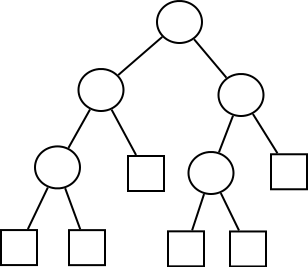
\includegraphics[width=\linewidth]{09/Grafik/img1.png}
\caption{Binärerbaum}
\end{wrapfigure}

\vspace{30pt}
\paragraph{Untere Schranke}
$t_{max} \geq \log_2(n!) = \Omega(n \log n) =  \log_2(n!) \leq t_{mean}$
\vspace{90pt}


\paragraph{Herleitung}
\[ \ln(n!) = \ln(n(n-1) \cdot (n-2) \cdot ... \cdot 2 \cdot 1) = \ln(n)+\ln(n-1)+...+1\]
\[ = \sum^{n}_{i=1} ln(i) \geq \int_1^n \ln(x) dx = \left[x\ln(x)-x \right]_1^{n} = n\ln(n)-n+1\]\\
\[\Rightarrow n! \geq e^{n\ln(n)-n+1} = e \cdot e^{-n} \cdot \left(e^{\ln(n)}\right)^n = e \cdot e^{-n} \cdot n = e\left(\frac{n}{e}\right)^n \] 
Stirling $n! \approx \sqrt{2 \pi n} (\frac{n}{e})^n$

%\newpage

\subsection{Lemma: Mittlere Tiefe der Blätter in einem Entscheidungsbaum $> \log_2(n)n$}

\paragraph{Beweis} Induktion nach m (Blattanzahl)

\begin{wrapfigure}[2]{l}{0.3\linewidth}
\vspace{-50pt}
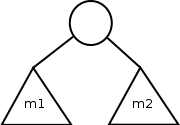
\includegraphics[width=\linewidth]{09/Grafik/img2.png}
\caption{Induktions-Ansatz}
\end{wrapfigure}

\vspace{30pt}
\paragraph{Untere Schranke}
$m_1, m_2 ~\hat{=}~$ Blattanzahl im linken bzw. rechten Teilbaum der Wurzel
\vspace{100pt}

\paragraph{Induktions Anfang:} $m=1 ~~~ t_{mean} = \log_2(1)=0$

\paragraph{Induktions Behauptung:} $t_{mean} \geq \log_2(m)$

\paragraph{Induktions Schritt:} Sei $m_1 < m, m_2 < m ~~~(1) ~\text{und}~ m_1+m_2=m ~~~(2)$ \\

b $~\hat{=}~$ Blatt im Entscheidungsbaum $T_b$\\
l $~\hat{=}~$ Blatt im linken Teilbaum $T_l$\\
r $~\hat{=}~$ Blatt im rechten Teilbaum $T_r$\\

\[t^{links}_{mean} \geq \log_2(m_1) ~~\text{und}~~t^{rechts}_{mean} \geq \log_2(m_2)\]

\[\frac{1}{m} \sum_{l} \cdot t_l = t^{links}_{mean}  \geq \log_2(m_1) \]

Verfahre analog für rechts.\\

\[\sum_b T_b = \sum_l (T_l+1) + \sum_r (T_r+1) \geq m_1+m_2 + m_1 \log_2(m_1) + m_2 \log_2(m_2) \]

Unter der Annahme, dass das Minimum bei $\frac{m}{2}$ liegt:
\[m_1 \log_2(m_1) + m_2 \log_2(m_2) \geq \frac{m}{2} \log_2 \left(\frac{m}{2} \right) \cdot 2 = m \log_2 \left(\frac{m}{2} \right) ~~~\text{mit (2)} \] 

Es folgt somit: 
\[ t_{mean} = \frac{1}{m} \sum_b T_b \geq  \frac{1}{m}\left(m+m\log_2\left( \frac{m}{2}\right)\right) = 1+ \log_2\left( \frac{m}{2}\right) = 1+ \log_2(m) -1 = \log_2(m) \]
\[q.e.d\]

%\newpage


\chapter{Radix-Sort}

\section{Beispiel:}
\begin{tabular}{l l l l}
  10\hly{1} & 0\hly{1}0 & \hly{1}00 & 001 \\
  01\hly{0} & 1\hly{0}0 & \hly{1}01 & 010\\
  00\hly{1} & 1\hly{1}0 & \hly{0}01 & 011 \\
  11\hly{1} & 1\hly{0}1 & \hly{0}10 & 100 \\
  10\hly{0} & 0\hly{0}1 & \hly{1}10 & 101 \\
  01\hly{1} & 1\hly{1}1 & \hly{1}11 & 110 \\
  11\hly{0} & 0\hly{1}1 & \hly{0}11 & 111 \\
\end{tabular}
\paragraph{Wichtig}Beginne die Sortierung mit dem niedrigsten Bit

\section{Pseudo-Code}
\lstinputlisting[language=Java, style = pseudo]{09/Code/radixsort.java}


\chapter{Binäre Suchbäume}

\paragraph{Zahlen} 12, 8, 3, 16, 24, 17, 10, 21, 14, 9 

\begin{figure}[H]
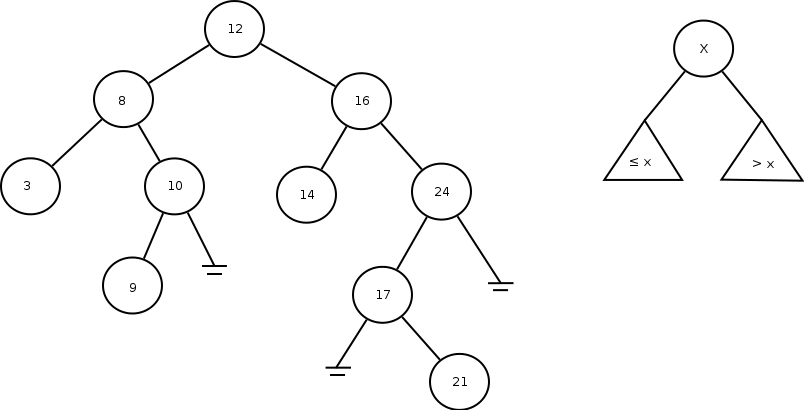
\includegraphics[width=\linewidth]{09/Grafik/img3.png}
\captionsetup{justification=raggedright, singlelinecheck=false}
\caption{Knotenorientierte Speicherung}
\end{figure}
